\begin{frame} \frametitle{The web Application}

	The web application performs the authentication as follows:
	
	\vfill

	\begin{itemize}
	 	\item Captures frames in a canvas.
	 	\item Analyzes them through the opencv's javascript\footnote{{ \color{red}
	 	\url{https://tinyurl.com/s2yprk7}}}.
	 	\item As the time one button is pressed, the canvas frame is sent to our
	 	server\footnote{{ \color{red} \url{https://biosys.casalinovalerio.com}}},
	 	which can register the face, or match the face with an already registered
	 	user.
	 	\item In the end, you can decide to be registered or you can query the
	 	system looking for a match of your face.
	\end{itemize}
	 
	\vfill

\end{frame}

\begin{frame} \frametitle{Does it work?}

	We actually did some \textbf{serious} testing on it. As you can
	clearly see in the picture below, it works!
	\begin{center}
		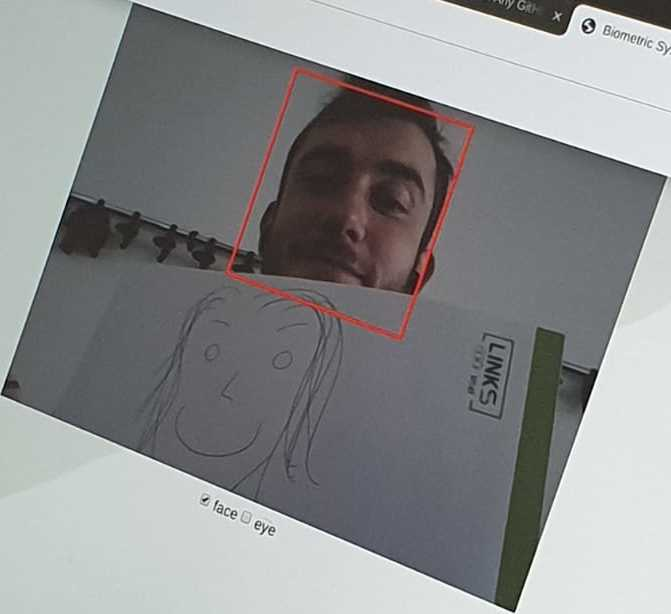
\includegraphics[width=.45\textwidth]{img/serious-testing}
	\end{center}
	

\end{frame}